\documentclass[10pt,twocolumn]{article}

\usepackage[letterpaper,margin=0.55in,columnsep=0.22in]{geometry}
\usepackage[T1]{fontenc}
\usepackage[utf8]{inputenc}
\usepackage{lmodern}
\usepackage{microtype}
\usepackage{amsmath}
\usepackage{booktabs}
\usepackage{longtable}
\usepackage{array}
\usepackage{tabularx}
\usepackage{graphicx}
\usepackage[font=small,labelfont=bf]{caption}
\usepackage{xcolor}
\usepackage{enumitem}
\usepackage{hyperref}
\usepackage{listings}
\Urlmuskip=0mu plus 1mu
\setlength{\parskip}{0.18em}
\setlength{\parindent}{0pt}
\setlength{\textfloatsep}{0.45em}
\setlength{\floatsep}{0.45em}
\setlength{\intextsep}{0.45em}
\setlength{\abovecaptionskip}{0.25em}
\setlength{\belowcaptionskip}{0.15em}
\setlength{\tabcolsep}{3.5pt}
\renewcommand{\arraystretch}{0.92}
\setlist[itemize]{topsep=0.2em,itemsep=0.08em,parsep=0pt}
\setlist[enumerate]{topsep=0.2em,itemsep=0.08em,parsep=0pt}

\hypersetup{
  colorlinks=true,
  linkcolor=black,
  urlcolor=blue,
  citecolor=black
}

\lstdefinestyle{cmd}{
  basicstyle=\ttfamily\scriptsize,
  columns=fullflexible,
  breaklines=true,
  frame=single,
  framerule=0.2pt,
  xleftmargin=0.02\linewidth,
  xrightmargin=0.02\linewidth
}

\newcommand{\weave}{WEAVE}
\newcommand{\dinos}{DINO-S}
\newcommand{\dinoc}{DINO-C}
\newcommand{\clips}{CLIP-S}

\title{\vspace{-1.0em}\textbf{Supplementary Material for WEAVE}\\
\large Reproducibility, Experimental Setup, and Artifact Ledger}
\author{Anonymous Authors}
\date{AAAI 2027 submission supplement}

\begin{document}
\maketitle

\begin{abstract}
This supplement gives the implementation and evaluation details needed to reproduce the
experiments reported in the main paper. It consolidates the paper source directory,
experiment records, frozen run configurations, training logs, evaluation summaries,
and timing records into a path-sanitized description. Machine-specific locations are
expressed as variables such as \texttt{<REPO\_ROOT>}, \texttt{<DATA\_ROOT>},
\texttt{<EXP\_ROOT>}, and \texttt{<CACHE\_ROOT>}; machine-specific paths are not
required by the protocol.
\end{abstract}

\section{Scope and Source of Record}

The main paper directory is \texttt{aaai2027\_v4}. The supplement is aligned with the
main-paper Table 1, Figure 5, and the method/ablation narrative current as of the AAAI v4
packet. The formal source of record is:
\begin{itemize}[leftmargin=1.5em,itemsep=0.2em]
  \item \path{aaai2027_v4/paper.tex}: main claims, tables, and captions.
  \item \path{aaai2027_v4/fig_data/dino_main.json}: DINO metric sidecar used by the figure scripts.
  \item \path{aaai2027_v4/fig_data/method_probes.json}: mechanism-probe sidecar.
  \item \path{experiments/architecture/hf_oriented_internal_early_stop.json}: D5 paper training configuration.
  \item \path{runs/submission/hf_oriented_internal_early_stop/config.json}: frozen merged run configuration.
  \item \path{runs/submission/hf_oriented_internal_early_stop/logs/training_*.csv}: training and internal-probe log.
  \item \path{exp/model_probe/inf_timing/generation_only_timing_summary.json}: generation-only timing record.
  \item \path{docs/model_probe/target_hf_delta_eval_summary.json}: aggregate target-HF route probe metrics.
  \item \path{docs/reproduction/internal_dynamics_early_stop.csv}: compact internal-dynamics curve.
\end{itemize}

All paths above are relative to \texttt{<REPO\_ROOT>/WEAVE}. All artifacts are referred to by logical paths so that the supplement
is portable across storage layouts.

\subsection{Directory Audit and Cleanup Policy}

Before writing this supplement, the paper directory and the full experiment tree were
audited rather than treated as a single opaque result folder. The audited
\texttt{exp} tree contained 111 experiment directories, 662 JSON files, 482 CSV files,
and 43 log files. The formal supplement only cites records that are needed to reproduce
the paper packet. Historical and failed experiments are retained in the ledger as
diagnostic context, but they are not used as source-of-truth for the main claims.
The source checkout was also audited and found to be an active research worktree
rather than a clean release tree: it contained hundreds of uncommitted deletions,
modifications, and untracked probe/supplement artifacts. For that reason, this supplement
uses committed paper files, frozen run snapshots, and explicit probe summary sidecars as
its source of record instead of relying on the ambient working-tree state.

\begin{figure}[t]
\centering

\includegraphics[width=0.48\linewidth]{supplement_figures/fig_exp_inventory.pdf}
\caption{Experiment inventory. Results used in the paper are separated from diagnostic
and historical runs retained for traceability.}
\label{fig:supp-exp-inventory}
\end{figure}

\begin{center}
\begin{tabularx}{\linewidth}{p{0.22\linewidth}rX}
\toprule
Group & Count & Interpretation \\
\midrule
Paper-facing runs & 5 & \texttt{dino\_s\_break}, \texttt{main\_table}, \texttt{bench\_all\_3060}, \texttt{other5\_eval}, and \texttt{latent\_wct\_baseline}. These are the directories used for the submission tables, timing, and supporting zero-shot checks. \\
Mechanism and infra probes & 5 & \texttt{model\_probe}, \texttt{infra\_diag}, \texttt{infra\_infer\_bench}, \texttt{infra\_opt}, and \texttt{param\_sweep}. These diagnose speed, target-HF routes, and inference knobs. \\
Ablation directories & 30 & \texttt{ablation\_*}, \texttt{abl\_*}, \texttt{sty\_inject}, and \texttt{seed3}. These support the causal claims but are not the final checkpoint source. \\
Historical search runs & 65 & Earlier \texttt{630\_*}, \texttt{710\_*}, \texttt{r3\_*}, \texttt{r4\_*}, \texttt{hp\_*}, \texttt{evo\_*}, and refactor runs. These explain design convergence and were excluded from the main result ledger unless explicitly referenced. \\
\bottomrule
\end{tabularx}
\end{center}

\paragraph{Cleanup rule.}
Raw records may contain machine-specific cache paths. The public supplement normalizes
all locations into four variables:
\begin{center}
\begin{tabularx}{\linewidth}{p{0.38\linewidth}X}
\toprule
Variable & Meaning \\
\midrule
\texttt{<REPO\_ROOT>} & Checkout containing \texttt{WEAVE}. \\
\texttt{<DATA\_ROOT>} & Dataset and latent-cache root. \\
\texttt{<EXP\_ROOT>} & Experiment output/checkpoint root. \\
\texttt{<CACHE\_ROOT>} & Evaluation feature-cache root. \\
\bottomrule
\end{tabularx}
\end{center}
No absolute paths, host addresses, machine names, or user names are needed to
run the protocol.

\begin{figure*}[t]
\centering

\includegraphics[width=0.86\textwidth]{supplement_figures/fig_repro_pipeline.pdf}
\caption{Reproducibility pipeline. The public protocol is defined by dataset artifacts,
the frozen config chain, the ordered evaluation boards, and metric sidecars. Physical
drive letters and host details are not part of the experiment definition.}
\label{fig:supp-repro-pipeline}
\end{figure*}

\subsection{Paper Directory Contents}

The \texttt{aaai2027\_v4} directory contains the submission source, generated figures,
figure sidecars, and build scripts. The 13 files in \texttt{fig\_data} are treated as
figure/data sidecars rather than raw experiment roots:

\begin{center}
\footnotesize
\begin{tabularx}{\linewidth}{p{0.32\linewidth}rX}
\toprule
File & Size & Role \\
\midrule
\path{dino_main.json} & 11175 & DINO-S/DINO-C sidecar for D5-512, P2A-256, and R5-WikiArt. \\
\path{method_probes.json} & 16354 & Aggregated mechanism-probe source for the method-probe figure. \\
\path{method_probes_run.log} & 16356 & Reproducibility log for probe aggregation. \\
\path{method_probe_endpoint.csv} & 2289 & Endpoint/AdaIN ablation values. \\
\path{method_probe_frequency.csv} & 3645 & Frequency/subband probe values. \\
\path{method_probe_style_separability.csv} & 415 & Style-separability probe values. \\
\path{swd_loss_separability.json} & 1074 & SWD-loss diagnostic sidecar. \\
\path{curve_metrics_hf.csv} & 19824 & Baseline curve metrics used for analysis plots. \\
\path{teaser_*.png/.jpg} & 295598 & Teaser visual assets for content, WEAVE, SaMam, Seedream, and StyleID. \\
\bottomrule
\end{tabularx}
\normalsize
\end{center}

The compiled paper figures are regenerated by the following scripts:
\path{gen_figures.ps1}, \path{plot_page1_summary.py},
\path{plot_method_probes.py}, and \path{make_radar_metric_blocks.py}. The supplement
does not depend on temporary LaTeX build files such as \path{paper.aux},
\path{paper.fls}, or prior compile logs.

\section{Datasets and Evaluation Boards}

\paragraph{D5-512.}
The primary benchmark is Distinct5-WikiArt at 512 px. It contains five WikiArt styles:
Early Renaissance, Impressionism, Minimalism, Rococo, and Ukiyo-e. Each style contributes
3600 training images and 150 test images. Evaluation uses all ordered source-target style
pairs with 30 content images per source style, giving 750 pairs in total. The 150
same-style pairs are retained as identity calibration rows rather than removed.

\paragraph{P2A-256.}
The photo-to-art board evaluates transfer at 256 px. It uses the same ordered evaluation
logic but with a lower-resolution latent/image cache. It is included to test whether the
method remains stable when high-frequency subbands are compressed by resolution.

\paragraph{R5-WikiArt.}
The broader WikiArt board evaluates style-family generalization. The full evaluation
space is all 20 WikiArt families with \(20 \times 20 \times 30 = 12000\) ordered pairs.
For the cross-method main table, external baselines are reported on the same 750-pair
subset, while the \weave{} checkpoint is also used to validate broader family coverage.

\begin{figure}[t]
\centering

\includegraphics[width=0.88\linewidth]{supplement_figures/fig_dataset_boards.pdf}
\caption{Evaluation-board construction. D5-512 and P2A-256 use 750-pair boards with
identity rows retained. R5-WikiArt expands the style-family space to 20 by 20 styles;
the main table uses the common 750-pair subset when comparing all methods.}
\label{fig:supp-dataset-boards}
\end{figure}

\paragraph{Pairing and calibration.}
All learned methods use the same ordered pair lists within a board. For D5-512 training,
source-target pairing uses the frozen pairing cache
\path{<DATA_ROOT>/wikiart_distinct5_samam_512_latents_ema/train/.latent_cache/prototype_pairing_top8.pt}.
The final paper run disables active top-\(k\) filtering at training time
(\texttt{pairing\_cache\_active\_topk=0}) after loading the cache. Identity rows are used
to estimate the no-op style floor and the content ceiling.

\subsection{Dataset Layout}

A reproducible installation should provide the following logical layout. The names are
shown as canonical relative roots; exact physical storage locations are intentionally
left variable.

\begin{center}
\footnotesize
\begin{tabularx}{\linewidth}{p{0.38\linewidth}X}
\toprule
Logical path & Contents \\
\midrule
\path{<DATA_ROOT>/wikiart_distinct5_samam_512_latents_ema/train} & Packed 512 px latent training cache for the five D5 styles, plus latent-cache metadata. \\
\path{<DATA_ROOT>/wikiart_distinct5_samam_512_latents_ema/train/.latent_cache/packed} & Packed latent tensors consumed by the training dataloader. \\
\path{<DATA_ROOT>/wikiart_distinct5_samam_512_classview/test} & D5-512 held-out class-view image tree used by full evaluation. \\
\path{<DATA_ROOT>/wikiart_distinct5_512_images/test} & D5-512 image tree used as a style-bank root for reference-feature cache generation. \\
\path{<DATA_ROOT>/wikiarts20_512_test} & R5-WikiArt reference/test tree. \\
\path{<DATA_ROOT>/p2a_256/...} & P2A-256 test/cache roots; use the same ordered-pair protocol and metric scripts as D5. \\
\bottomrule
\end{tabularx}
\normalsize
\end{center}

\paragraph{Expected counts.}
For D5-512, the evaluation board has 5 source styles, 5 target styles, and 30 content
images per source style, for 750 ordered evaluations. For P2A-256, identity-style rows
are retained in the board definition but some external baselines only provide the 600
off-diagonal transfers; this is why DINO sidecars record both \texttt{n\_images} and
\texttt{n\_skipped}. For R5-WikiArt, the full board is 12000 pairs, while the main table
uses the common 750-pair subset for cross-method comparison.

\subsection{Data Preprocessing Contract}

Training consumes latent tensors rather than raw images. A correct preprocessing run must:
\begin{enumerate}[leftmargin=1.6em,itemsep=0.2em]
  \item Resize/crop images consistently with the target board resolution.
  \item Encode images with the SD1.5 EMA VAE and store the latent scaling factor
  \texttt{0.18215} in the config path.
  \item Preserve style subdirectories exactly as listed in the config:
  \texttt{Early\_Renaissance}, \texttt{Impressionism}, \texttt{Minimalism},
  \texttt{Rococo}, and \texttt{Ukiyo\_e}.
  \item Build or provide the prototype pairing cache used by D5 training.
  \item Build CLIP/DINO reference caches under \texttt{<CACHE\_ROOT>} only from held-out
  test/style-bank images, not from generated outputs.
\end{enumerate}

The public result is reproducible as long as these logical artifacts match. Their
physical drive letters and cache locations are not part of the method.

\paragraph{Dataset integrity checks.}
The dataloader assumes every style directory contains latent tensors encoded with the
same VAE, style labels are derived from directory names, and the train/test split is not
mixed. A minimal integrity pass should check style directory names, count consistency,
latent tensor shape and scale, absence of generated images in reference caches, and
whether the pairing cache was built from training latents rather than held-out test
images. If a dataset is moved, only root paths should change; style names, cache names,
and board construction should remain byte-identical or be regenerated from the same
scripts.

\section{Hardware and Software Environment}

All training and timing numbers reported in the paper come from a single consumer-class
GPU. The environment is described by role, not by machine identifier:

\begin{center}
\begin{tabularx}{\linewidth}{p{0.38\linewidth}X}
\toprule
Component & Value \\
\midrule
GPU class & NVIDIA GeForce RTX 3060, 12\,GB \\
Training precision & bfloat16 automatic mixed precision \\
TF32 matmul & enabled \\
Device count & 1 GPU \\
\bottomrule
\end{tabularx}
\end{center}

The method itself does not depend on a specific software stack version beyond the ranges listed above; any
consumer GPU with $\geq 12$\,GB VRAM and a working PyTorch CUDA build reproduces the
reported numbers.

The software stack follows \texttt{WEAVE/requirements.txt}: PyTorch
\(\ge 2.3\), torchvision \(\ge 0.18\), transformers \(4.57 \le v < 5\), diffusers
\(0.38 \le v < 0.39\), LPIPS, torchmetrics, torch-fidelity, Pillow, NumPy, SciPy,
scikit-learn, and tqdm. The frozen VAE is the SD1.5 EMA VAE used only for latent
encoding/decoding; it contributes 84M frozen parameters and is not trained.

\section{Model and Training Setup}

\weave{} trains a compact velocity model in SD1.5 VAE latent space. A single-level Haar
DWT splits the latent into LL/LH/HL/HH subbands. The base network has four residual blocks
of width 64 and three supervised output heads for LL/LH/HL. The D5 model adds separate
pooled target-LH and target-HL encoders whose gated residuals enter only the matching
velocity heads. The complete model has 1,037,087 trainable parameters; the frozen VAE is
reported separately as \(1.04\mathrm{M}^{+84\mathrm{M}}\).

\begin{center}
\begin{tabularx}{\linewidth}{p{0.38\linewidth}X}
\toprule
Field & Paper configuration \\
\midrule
Config & \path{experiments/architecture/hf_oriented_internal_early_stop.json} \\
Base config & \path{config.json} \\
Seed & 42 \\
Maximum epochs & 15; internal stop at epoch 4 \\
Batch size & 96 \\
Gradient accumulation & 1 \\
Optimizer & AdamW, fused when available \\
Learning rate & \(2.0 \times 10^{-4}\) \\
Minimum learning rate & \(1.0 \times 10^{-5}\) \\
Schedule & cosine \\
Weight decay & \(1.0 \times 10^{-4}\) \\
Gradient clipping & 1.0 \\
Precision & bf16 AMP \\
Channels-last layout & enabled \\
Torch compile & disabled \\
Workers & 0 \\
Checkpoint interval & every epoch \\
Internal probe batch & 4 fixed latents at (t=0.5) \\
\bottomrule
\end{tabularx}
\end{center}

The structure-aligned target is constructed in the wavelet basis. The LL target is a mild
content-preserving blend,
\[
  \mathrm{LL}_{target} = 0.7\,\mathrm{LL}_{content}
  + 0.3\,\mathrm{AdaIN}(\mathrm{LL}_{content}, \mathrm{LL}_{style}),
\]
while the high-frequency target uses the target-style LH/HL/HH bands. The implementation
minimizes the band-weighted velocity-matching loss given in the main paper; no additional edge
or low-pass loss is active in the submitted configuration.

\subsection{Resolved Configuration Details}

The frozen merged configuration for the paper run resolves the short public config
into the following relevant fields:

\begin{table*}[t]
\centering
\footnotesize
\begin{tabularx}{\textwidth}{p{0.30\textwidth}p{0.16\textwidth}X}
\toprule
Field & Value & Relevance \\
\midrule
\texttt{model.contract\_family} & \texttt{weave} & Selects the WEAVE architecture contract. \\
\texttt{model.base\_dim} & 64 & Backbone width. \\
\texttt{model.time\_dim} & 256 & Time embedding width. \\
\texttt{model.num\_res\_blocks} & 4 & Main residual block count. \\
\texttt{model.num\_hires\_blocks} & 2 & High-resolution block count. \\
\texttt{model.num\_decoder\_blocks} & 2 & Decoder block count. \\
\texttt{model.target\_latent\_hf\_subband\_fusion\_enabled} & true & Activates orientation-specific target-HF residuals. \\
\texttt{model.target\_latent\_hf\_head\_fusion\_gate\_init} & 0.18 & Initial LH/HL route gate. \\
\texttt{model.lowpass\_mode} & \texttt{dwt\_haar} & Single-level Haar decomposition. \\
\texttt{model.endpoint\_adain\_mode} & \texttt{spatial\_fiber} & High-frequency residual statistics matched after every Euler step. \\
\texttt{model.endpoint\_adain\_only\_last\_step} & false & Keeps AdaIN inside all eight integration updates. \\
\texttt{model.endpoint\_adain\_scale} & 2.0 & Inference-time extrapolation toward matched statistics. \\
\texttt{model.style\_extrap\_alpha} & 0.1 & Slight target-statistics extrapolation at inference. \\
\texttt{bridge.objective\_mode} & \texttt{flow\_matching} & Noise-regularized endpoint-velocity regression. \\
\texttt{bridge.loss\_type} & \texttt{mse} & Velocity matching loss. \\
training path & $t\sim\mathcal U[0,1]$ & Time sampling used by the submitted flow objective. \\
\texttt{bridge.bridge\_sigma} & 0.02 & Scales the $\sqrt{t(1-t)}$ interpolation perturbation. \\
\texttt{bridge.training\_target\_projection\_mode} & \texttt{dwt} & Target construction in wavelet space. \\
\texttt{bridge.spectral\_w\_ll/lh/hl/hh} & 0.3/1.0/1.0/inactive & HH has no velocity head in WEAVE. \\
\texttt{bridge.ll\_partial\_alpha} & 0.3 & Mild LL style-statistics migration. \\
\texttt{training.internal\_probe\_enabled} & true & Measures fixed-batch loss-path gradients after each epoch. \\
\texttt{training.internal\_early\_stop\_enabled} & true & Stops at the first gate/gradient transition. \\
\bottomrule
\end{tabularx}
\caption{Resolved fields from the frozen paper configuration.}
\label{tab:supp-resolved-config}
\normalsize
\end{table*}

\subsection{Training Log Audit}

The D5 paper run contains four logged epochs, each with 52 optimizer steps and effective
batch size 96. The wall-clock epoch time sums to 82.80 s. The probe is evaluated after the
optimizer and scheduler step, before checkpoint saving, and does not decode images.

\begin{center}
\footnotesize
\begin{tabular}{rrrrr}
\toprule
Epoch & Loss & Learning rate & Epoch time (s) & Stop event \\
\midrule
1 & 1.3631 & 2.0000e-4 & 25.72 & no \\
2 & 1.3318 & 1.9792e-4 & 19.23 & no \\
3 & 1.3199 & 1.9179e-4 & 18.94 & no \\
4 & 1.2499 & 1.8186e-4 & 18.90 & yes \\
\bottomrule
\end{tabular}
\normalsize
\end{center}

The first epoch is slower because caches and kernels are warmed. Later epochs take about
19 s on a single RTX 3060 (12\,GB), including the fixed-latent probe.

\subsection{Internal-Dynamics Probe}

For a fixed latent minibatch, the implementation performs one backward pass for the LL
loss and one for the summed LH/HL loss. Gradients are aggregated over the shared input,
attention, AdaLN, and feed-forward modules. The target-HF route and ordinary HF heads are
measured separately. The model runs in evaluation mode during the probe, no optimizer step
is taken, and \texttt{torch.random.fork\_rng} restores CPU and CUDA random states.

\begin{center}
\footnotesize
\begin{tabular}{rrrrrr}
\toprule
Epoch & Mean gate & Gate delta & Shared LL/HF & Route/shared HF & Route/HF head \\
\midrule
1 & 0.173068 & 0.000000 & 1.4727 & 0.8323 & 0.1816 \\
2 & 0.172264 & -0.000803 & 1.4328 & 0.6133 & 0.1907 \\
3 & 0.172009 & -0.000255 & 1.0868 & 0.4984 & 0.2111 \\
4 & 0.175719 & +0.003710 & 0.1634 & 0.2370 & 0.4561 \\
\bottomrule
\end{tabular}
\normalsize
\end{center}

Epoch 4 is the first joint event where the gate derivative is positive and the shared
LL/HF ratio contracts by at least 35\% from the preceding epoch. A retrospective probe of the complete 15-epoch curve selects
the same epoch, whose DINO-S is the curve maximum. Residual alignment to the FM target,
however, continues to improve after epoch 4 while DINO-S declines. This separates the
proposed transition from ordinary loss-based early stopping: it detects a change in route
ownership rather than a plateau in endpoint regression.

The original absolute crossing-at-one rule was scale-sensitive. Replacing it by
$\rho_e/(\rho_{e-1}+\epsilon)\leq0.65$ selects epoch 4 for probe batches 2/4/8 and seeds
42/7, and epoch 3 for seed 123. The additional seed-7 and seed-123 checkpoints give
(DINO-S, CLIP-S, LPIPS, DINO-C) of (0.4910, 0.7140, 0.2668, 0.8076) and
(0.4862, 0.7144, 0.2552, 0.8040), respectively. Thus the event is stable to the tested
probe scale and keeps the selected point near the canonical frontier; it is not claimed as
an architecture-independent criterion.

\begin{figure}[t]
\centering

\includegraphics[width=0.9\linewidth]{supplement_figures/fig_training_audit.pdf}
\caption{Training dynamics for the selected D5-512 checkpoint. Training stops at
epoch 4 when the high-frequency conditioning gates increase and the shared LL/HF gradient ratio
contracts sharply relative to the preceding epoch.}
\label{fig:supp-training-audit}
\end{figure}

\subsection{Implementation Notes}

The implementation is organized around \path{run.py} for training,
\path{trainer.py} for the optimization loop, \path{model.py} for the compact
velocity network, \path{wavelet.py} for DWT/IDWT operations, and
\path{utils/run_evaluation.py} for board evaluation. Each training run copies
a source snapshot into the run directory; this is why the paper checkpoint can be audited
independently of later code cleanup.

\begin{center}
\footnotesize
\begin{tabularx}{\linewidth}{p{0.33\linewidth}X}
\toprule
Module & Reproducibility role \\
\midrule
\path{run.py} & Loads resolved config, seeds the run, builds dataloader, launches trainer, and optionally invokes full evaluation. \\
\path{trainer.py} & Implements optimization, fixed-batch internal probes, checkpoint snapshots, and epoch logs. \\
\path{internal_dynamics.py} & Measures route-specific gradients and applies the gate/gradient transition rule. \\
\path{model.py} & Defines the WEAVE velocity backbone, oriented target-HF route, heads, solver hooks, and endpoint operations. \\
\path{wavelet.py} & Implements Haar DWT/IDWT and subband packing/unpacking used by training and inference. \\
\path{utils/run_evaluation.py} & Generates ordered board outputs, decodes VAE latents, builds/loads caches, computes CLIP/LPIPS, and writes summaries. \\
\path{aaai2027_v4/*.py} & Converts sidecars into paper figures and supplement plots. \\
\bottomrule
\end{tabularx}
\normalsize
\end{center}

Implementation details that materially affect reproduction are:
\begin{itemize}
  \item \textbf{Latent scale:} the VAE latent scale factor is \texttt{0.18215}.
  \item \textbf{Subband contract:} LL carries structure/color anchor information, while
  LH/HL/HH carry high-frequency style statistics.
  \item \textbf{Prediction target:} training predicts latent-space velocity/endpoint
  transport rather than RGB pixels.
  \item \textbf{Output heads:} the compact network supervises LL/LH/HL heads in the
  audited paper config. HH participates in target/statistics construction and endpoint
  alignment.
  \item \textbf{Evaluation separation:} generation, VAE decode, CPU image materialization,
  CLIP/DINO/LPIPS metrics, and CSV writing are timed separately.
  \item \textbf{Cache safety:} reference feature caches are derived from held-out style
  banks and may be rebuilt; they should not be copied from generated-output folders.
\end{itemize}

\section{Information-Flow Diagnosis}

The probe campaign was designed to answer a narrower question than the main table:
whether the model's weak style movement came from a wrong target, insufficient training
time, or a disconnected conditioning path. The diagnosis favors the third explanation.
The structure-aligned target already asks for style in the high-frequency bands:
\[
  \begin{array}{l}
  \mathrm{LL}_{target}=0.7\,\mathrm{LL}_{content}
  +0.3\,\mathrm{AdaIN}(\mathrm{LL}_{content},\mathrm{LL}_{style}),\\
  \mathrm{LH/HL/HH}_{target}=\mathrm{LH/HL/HH}_{style}.
  \end{array}
\]
Thus the loss is not merely reconstructing the source image. The failure mode is that,
in the baseline, the target image latent is used to construct supervision but does not
strongly enter the velocity predictor as an image-specific condition.

\begin{center}
\footnotesize
\begin{tabularx}{\linewidth}{p{0.26\linewidth}p{0.30\linewidth}X}
\toprule
Route & Signal path & Probe reading \\
\midrule
Baseline style memory & \texttt{style\_id} \(\rightarrow\) style memory \(\rightarrow\) cross-attention & Coarse style prior. Gates stay near 0.056--0.061, but removing this route hurts full metrics, so it is useful but not sufficient. \\
Global target-token fusion & target latent \(\rightarrow\) all style tokens \(\rightarrow\) backbone & Connected but too global; it over-controls LL and does not improve useful style transfer. \\
Raw spatial target-HF & target DWT-HF maps \(\rightarrow\) HF residual maps & Has sufficient capacity, but leaks target geometry and collapses content. \\
Pooled subband target-HF & target DWT-HF \(\rightarrow\) per-subband pooled code \(\rightarrow\) HF residual velocity & Current usable path: stronger style signal without target-coordinate leakage. \\
\bottomrule
\end{tabularx}
\normalsize
\end{center}

The strongest negative control is the raw spatial target-HF route. It raises \dinos{}
and \clips{}, which shows that the network can read target-style information when the
path is opened. However, the same run reduces \dinoc{} to 0.4043 and raises LPIPS to
0.5382, so the gain is not a valid style-transfer improvement. It is target-layout
leakage. The accepted route therefore compresses target high frequencies into
coordinate-free subband codes before they reach the HF velocity heads.

\subsection{Probe Protocol and Result Ledger}

All probe rows below fine-tune from the same \texttt{brk\_a\_ll03\_10ep} checkpoint
family and are evaluated on the D5-512 board with the canonical DINOv2-small metrics.
The rows are diagnostic architecture probes; they are not mixed into the main table
unless the corresponding architecture is fully rerun under the paper protocol.

\begin{center}
\scriptsize
\resizebox{\linewidth}{!}{%
\begin{tabular}{lrrrrrp{0.36\linewidth}}
\toprule
Run & \dinos{} & \dinoc{} & LPIPS & \clips{} & Off-\dinos{} & Verdict \\
\midrule
\texttt{target\_hf\_delta\_ft15, ep6} & 0.4827 & 0.7917 & 0.2950 & 0.7175 & 0.3986 & Path connected, but modest. \\
\texttt{target\_hf\_delta\_ft15, ep15} & 0.4825 & 0.7913 & 0.2991 & 0.7180 & 0.3987 & Longer fine-tune does not solve the bottleneck. \\
\texttt{target\_hf\_delta\_strong\_ft6} & 0.4870 & 0.7991 & 0.2955 & 0.7176 & 0.4019 & First usable HF route. \\
\texttt{target\_hf\_spatial\_ft6} & 0.4901 & 0.4043 & 0.5382 & 0.7483 & -- & Reject: target geometry leak. \\
\texttt{target\_hf\_subband\_ft6} & \textbf{0.4886} & 0.7981 & 0.2966 & \textbf{0.7209} & 0.4039 & Primary current architecture probe. \\
\texttt{subband residual ablated} & 0.4858 & 0.7888 & 0.3010 & 0.7205 & 0.4033 & Same checkpoint, target-HF residuals zeroed at inference. \\
\texttt{subband residual 1.25x} & 0.4873 & 0.7887 & 0.3007 & 0.7201 & 0.4045 & Slight off-style gain but lower balanced metrics. \\
\texttt{subband residual 1.5x} & 0.4875 & 0.7798 & 0.3054 & 0.7211 & 0.4067 & Style-biased; content cost too high. \\
\texttt{subband residual HH 1.5x} & 0.4878 & 0.7836 & 0.3034 & 0.7206 & 0.4061 & HH-only boost still trades content for off-style. \\
\texttt{target\_hf\_hybrid\_ft6} & 0.4858 & 0.7978 & 0.2956 & 0.7197 & 0.4010 & Extra shared/residual mixing does not help. \\
\texttt{target\_hf\_subband\_head\_ft6} & 0.4873 & 0.7987 & 0.2962 & 0.7192 & 0.4021 & Safe, but below subband residual. \\
\texttt{target\_hf\_spatial\_energy\_ft6} & 0.4861 & 0.7909 & 0.2978 & 0.7204 & 0.4027 & Content cost without headline gain. \\
\texttt{target\_hf\_texture\_ft6} & 0.4860 & 0.7980 & 0.2964 & 0.7182 & 0.4013 & Stationary stats are safe but weak alone. \\
\texttt{target\_hf\_subband\_texture\_ft6} & 0.4884 & \textbf{0.7988} & \textbf{0.2960} & 0.7194 & \textbf{0.4043} & Conservative alternate with best off-style/content balance. \\
\texttt{target\_hf\_content\_anchor\_ft6} & 0.4844 & 0.7955 & 0.2982 & 0.7173 & 0.3995 & Safe placement, not competitive. \\
\texttt{target\_hf\_multitoken\_ft6} & 0.4836 & 0.7941 & 0.2980 & 0.7187 & 0.3988 & More stationary-stat tokens do not help. \\
\texttt{target\_hf\_subband\_deep\_energy\_ft6} & 0.4826 & 0.7949 & 0.2975 & 0.7176 & 0.3977 & Deeper energy-normalized residual is worse. \\
\texttt{target\_hf\_subband\_film\_head\_ft6} & 0.4826 & 0.7917 & 0.2996 & 0.7180 & 0.3983 & Direct FiLM into HF heads disturbs the pretrained field. \\
\texttt{target\_hf\_subband\_basis\_ft6} & 0.4828 & 0.7937 & 0.2971 & 0.7183 & 0.3986 & Low-rank content-derived basis is safe but underpowered. \\
\texttt{target\_hf\_subband\_pairstats\_ft6} & 0.4838 & 0.7943 & 0.2971 & 0.7183 & 0.3994 & Current-target global HF statistics are too coarse. \\
\texttt{target\_hf\_subband\_diraux\_ft6} & 0.4862 & 0.7939 & 0.2974 & 0.7189 & 0.4021 & Direction auxiliary improves the probe but hurts image metrics. \\
\texttt{subband residual time windows} & 0.4866 & 0.7936 & 0.2975 & 0.7194 & 0.4026 & Early/late normalized windows both underperform full residual. \\
\texttt{target\_hf\_subband\_nomem\_ft6} & 0.4849 & 0.7948 & \textbf{0.2943} & 0.7167 & 0.4013 & Removing style memory cleans the probe route but weakens style/content metrics. \\
\texttt{target\_hf\_subband\_memres\_ft6} & 0.4866 & 0.7935 & 0.2977 & 0.7192 & 0.4025 & Explicit style-memory prior subtraction is below subband-only. \\
\bottomrule
\end{tabular}}
\normalsize
\end{center}

Two implementation lessons follow from the probes. First, any promoted target-HF
architecture should supervise an HH output path when HH appears in the target. Otherwise
the target contains information that no model head can directly predict. Second, more
training by itself is not the primary lever: the 15-epoch HF-delta curve remains below
the 6-epoch subband route. The useful capacity is frequency-specific and route-specific,
not merely total wall-clock exposure.

A matched inference-time ablation further checks that the subband route is causal rather
than incidental. Using the trained subband checkpoint, we zero only the three target-HF
subband residual modules during evaluation. This lowers \dinos{} from 0.4886 to 0.4858,
\dinoc{} from 0.7981 to 0.7888, and worsens LPIPS from 0.2966 to 0.3010. Thus the
learned residual path contributes to both style transfer and content-compatible HF
transport; it is not a dead branch and not merely a style-over-content shortcut.
Scaling the same residual to 1.25x or 1.5x does not improve the balanced point:
off-\dinos{} and \clips{} can increase, but \dinos{}, \dinoc{}, and LPIPS worsen.
The useful target-HF route is therefore not simply amplitude-limited; the next
architecture needs better residual direction or conditioning rather than a scalar gain.
This is supported by a direct residual-direction probe: the residual lowers the
training-target HF MSE, but its average cosine to the ideal correction direction is only
0.158 and about 98.2\% of its energy is orthogonal to that direction. HH is the most
aligned band, yet HH-only amplification still follows the same content-cost trend.
A direct training auxiliary that aligns the residual to
\(\mathrm{stopgrad}(v^\star_{\mathrm{HF}}-v_{\mathrm{base}})\) increases the
probe cosine to 0.322 and the MSE-improvement fraction to 0.117, but lowers
\dinos{} to 0.4862 and also worsens \dinoc{}, \clips{}, and LPIPS. Therefore the
direction gap is real, but a separate residual-direction loss is too intrusive in the
current transport field.
An inference-only time-window probe also rejects the idea that this residual should
be moved to only early or only late ODE steps. With normalized half-trajectory windows,
early-only and late-only residuals both give \dinos{} around 0.4866 and lower
\dinoc{} around 0.7936, below the full residual. Thus the branch is not merely a late
texture patch; it should remain a small full-path correction while its basis or
conditioning is improved.

A low-rank content-basis variant further tested whether the target-HF code should only
select coefficients over residual bases produced from content features. This design
disconnects target spatial coordinates, but it lowers \dinos{} to 0.4828 and
off-\dinos{} to 0.3986. The result indicates that the current bottleneck is not solved
by making the residual basis more restrictive; the target-HF route still needs enough
image-specific orientation and texture capacity.

A pairwise-statistics variant added coordinate-free statistics of the current HF state,
the target HF state, and their difference to the per-subband target-HF code. This tests
whether the residual needs an explicit ``how far from target statistics'' signal.
The run remains content-safe but lowers \dinos{} to 0.4838 and off-\dinos{} to 0.3994.
Thus global current-target discrepancy descriptors are too coarse for this route; the
simple target-only subband code remains the stronger conditioning signal.

The no-memory probe clarifies the role of the style-memory branch. Disabling generic
style-memory cross-attention makes the target-HF path easier to read in gradients and
aligns auxiliary HF-statistic gradients with the HF-MSE objective, but full evaluation
drops \dinos{}, \dinoc{}, \clips{}, and off-\dinos{} relative to the subband route.
The visual grid also shows over-smoothed transfers in the Minimalism target column.
Thus the remaining design problem is not to delete style memory; it is to keep style
memory as a bounded category-level prior while letting target-HF subband codes carry
the image-specific residual style.

A follow-up memory-residualized route tested explicit subtraction of a learned
style-memory prior from the per-subband target-HF code. It recovered part of the
no-memory loss but still trailed the plain subband route on \dinos{}, \dinoc{},
\clips{}, LPIPS, and off-\dinos{}. This negative result argues against algebraically
removing the memory prior; future routes should regularize or measure route usage
without perturbing the useful category prior.

\section{Inference Setup}

The main paper uses an 8-step Euler solver. Spatial-fiber AdaIN is applied to the
high-frequency residual after every solver step. The main D5-512 row uses
\path{runs/submission/hf_oriented_internal_early_stop/epoch_0004.pt}. P2A and R5 use the
audited base-WEAVE checkpoints reported before the oriented D5 route was enabled.

\begin{center}
\footnotesize
\begin{tabularx}{\linewidth}{p{0.42\linewidth}X}
\toprule
Inference field & Value \\
\midrule
ODE solver & Euler \\
ODE steps & 8 \\
Evaluation batch size & 2 for D5-512 generation timing \\
VAE decode batch size & 16 in the timing script \\
Spatial-fiber AdaIN & every Euler step, scale 2.0 \\
Style extrapolation & \(\alpha_{\mathrm{extrap}}=0.1\) \\
Generated-image count for timing & 750 \\
Timing column & generation only, metrics excluded \\
\bottomrule
\end{tabularx}
\normalsize
\end{center}

\subsection{Evaluation Runtime Anatomy}

The paper reports the measured generation-only time for the selected D5 checkpoint:
126.00\,s for 750 images on one RTX 3060 (12\,GB). This timing includes the 8-step
trajectory and VAE decoding, but excludes latent caching, metric extraction, and result
serialization. We do not reuse component traces from earlier checkpoints because they do
not describe the selected model.

\begin{figure}[t]
\centering
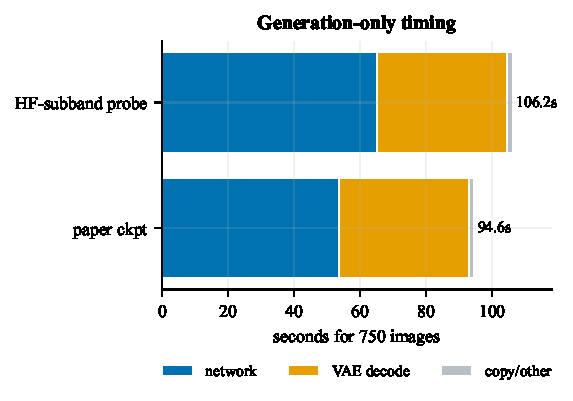
\includegraphics[width=0.56\linewidth]{supplement_figures/fig_timing_breakdown.pdf}
\caption{Generation-only time for the selected WEAVE checkpoint on a single RTX 3060
(12\,GB): 126.00\,s for 750 images. Latent caching and metric computation are excluded.}
\label{fig:supp-timing}
\end{figure}

\subsection{Inference Variants}

The following older base-WEAVE variants share one checkpoint and differ only in
inference-time stepwise AdaIN strength. They remain diagnostic operating points and are
not the updated main D5 result.

\begin{table*}[t]
\centering
\footnotesize
\begin{tabularx}{\textwidth}{lrrrrX}
\toprule
Variant & Scale & \dinos{} & \clips{} & LPIPS & Use \\
\midrule
\texttt{WEAVE-m} & 1.5 & 0.4843 & 0.7180 & 0.2925 & Balanced diagnostic point. \\
\texttt{WEAVE-s} & 1.6 & 0.4845 & 0.7179 & 0.2867 & Peak average of DINO-S and CLIP-S. \\
\texttt{WEAVE-q} & 2.0 & 0.4859 & 0.7075 & 0.2583 & Previous base-WEAVE max-DINO diagnostic. \\
\bottomrule
\end{tabularx}
\caption{Alternative inference settings evaluated from the same base checkpoint.}
\label{tab:supp-inference-variants}
\end{table*}

The audited generation-only timing for the selected checkpoint on a single RTX 3060
(12\,GB) is:

\begin{center}
\begin{tabular}{lr}
\toprule
Timing field & Value \\
\midrule
Total generation-only wall clock & 126.00 s \\
Images & 750 \\
Wall time per image & 168.00 ms \\
\bottomrule
\end{tabular}
\end{center}

\section{Metrics}

\paragraph{\dinos.}
\dinos{} is the primary style metric. It is the cosine similarity between the DINOv2-small
CLS feature of the generated image and the nearest reference feature in the target-style
reference pool. The source image is excluded from the reference pool when applicable.

\paragraph{\clips.}
\clips{} is the secondary style metric, computed as CLIP ViT-B/32 image-feature cosine
similarity to the target-style reference prototype.

\paragraph{\dinoc.}
\dinoc{} measures content preservation as DINOv2-small CLS cosine similarity between the
generated image and the source image.

\paragraph{LPIPS.}
LPIPS uses the AlexNet backbone and is reported as a lower-is-better content distance.
Radar plots display \(1-\mathrm{LPIPS}\) so all axes point outward for better values.

\subsection{IDT--TGT Evaluation Guideline}

The guideline adds two source-independent reference outputs to the ordinary metric table.
For a request with source image $x$ and target style $s$, define
\begin{equation}
  y_{\mathrm{IDT}}(x,s)=x,
  \qquad
  y_{\mathrm{TGT}}(x,s)=r_s,
\end{equation}
where $r_s$ is a fixed image from the held-out reference pool for style $s$. The D5
implementation selects the first image in the deterministic reference order and reuses it
for every source paired with that target style. Thus TGT depends on the requested style but
not on source content. It is an evaluation control, not an input to \weave{} or any baseline.

\paragraph{Why two references are needed.}
IDT represents a no-op: it preserves all source content but makes no requested edit. A
method should therefore score above IDT on \dinos{} and \clips{} before a low LPIPS can be
read as successful transfer. TGT represents the opposite extreme: it has the requested
style but unrelated content. A content-preserving method should have lower LPIPS and higher
\dinoc{} than TGT. The intuitive acceptable region is therefore bracketed by
\begin{equation}
\begin{aligned}
M_{\mathrm{style}}(y)&>M_{\mathrm{style}}(y_{\mathrm{IDT}}),\\
\mathrm{LPIPS}(y,x)&<\mathrm{LPIPS}(y_{\mathrm{TGT}},x),\\
\mathrm{DINO\text{-}C}(y,x)&>\mathrm{DINO\text{-}C}(y_{\mathrm{TGT}},x).
\end{aligned}
\end{equation}
We inspect the inequalities separately and do not combine them into a weighted score.

\paragraph{Interpretation and scope.}
IDT and TGT are empirical anchors, not mathematical bounds: a generated image may score
outside either reference because the metrics are imperfect. Crossing IDT in the wrong
direction indicates style suppression under that metric. Moving beyond TGT in content
distance identifies a content-loss regime relative to a deliberately unrelated target-style
image. This is a prompt for visual inspection, not a verdict on the method outside the
current board and metric. On D5-512, IDT
is (\dinos{} 0.419, \clips{} 0.693, LPIPS 0, \dinoc{} 1), while TGT is
(1.000, 0.863, 0.776, 0.215). TGT reaches \dinos{} 1.000 because the selected reference is
part of the same target-style feature pool used by that metric; this value is expected and
should not be read as model performance.

Using each of the first five deterministic target exemplars changes TGT LPIPS from 0.752
to 0.783 and \dinoc{} from 0.189 to 0.246. StyleAligned remains beyond every TGT LPIPS
anchor (0.869), so the content-collapse diagnosis is not determined by the first exemplar.

\subsection{Metric Cache and Determinism}

Evaluation uses deterministic seeds and cached reference features. Cache entries are
logical artifacts under \path{<CACHE_ROOT>/eval_cache}; they may be rebuilt as long as
the image roots and model backbones are unchanged. The full-eval summaries record:
\begin{itemize}[leftmargin=1.5em,itemsep=0.2em]
  \item CLIP backend: HuggingFace transformers backend.
  \item LPIPS network: AlexNet.
  \item Reference-cache limit per style: 16 for the paper full-eval records.
  \item Source-feature cache: one cache per board/image-size setting.
  \item Metric postprocessing: disabled for the main records.
\end{itemize}

\subsection{DINO Sidecar Coverage}

The DINO sidecar contains 37 board-method entries. D5-512 and P2A-256 each include 13
methods: Identity, SD-Turbo, StyleAligned, Z-STAR, StyleShot, CUT, SaMST, SaMam,
Seedream 4.5, Latent-WCT/WCT, StyleID, AdaIN, and \weave{} as applicable. R5-WikiArt
contains 11 entries because not every diagnostic baseline was rerun on the R5 board.
The paper table is manually aligned to these sidecars and the CLIP/LPIPS summaries.

\paragraph{Metric interpretation caveats.}
\dinos{} and \clips{} are style-reference similarities, not human preference labels.
\dinoc{} and LPIPS quantify source preservation, but they penalize different failure
modes: LPIPS is sensitive to perceptual pixel/feature distance, whereas \dinoc{} is a
semantic feature similarity. The paper therefore treats the result as a multi-objective
operating point. A method with high \dinos{} and very high LPIPS is not considered a
content-preserving transfer method even if it appears strong on style alone.

\section{Main Results Used by the Paper}

The main table reports the following \weave{} rows:

\begin{center}
\begin{tabular}{lrrrr}
\toprule
Board & \dinos{} & \clips{} & LPIPS & \dinoc{} \\
\midrule
D5-512 (oriented HF) & 0.4918 & 0.7128 & 0.2595 & 0.8102 \\
P2A-256 & 0.4801 & 0.6681 & 0.3116 & 0.8612 \\
R5-WikiArt & 0.5226 & 0.7747 & 0.2895 & 0.7717 \\
\bottomrule
\end{tabular}
\end{center}

\begin{table*}[t]
\centering
\scriptsize
\setlength{\tabcolsep}{2.0pt}
\caption{Full comparison ledger used by the main paper. Higher DINO-S, CLIP-S, and
DINO-C and lower LPIPS are better. Dashes mark unavailable or withheld
metadata rather than inferred values.}
\label{tab:supp-full-main}
\resizebox{\textwidth}{!}{%
\begin{tabular}{lrrrrrrrrrrrrrrr}
\toprule
Method & \multicolumn{4}{c}{D5-512} & \multicolumn{4}{c}{P2A-256} & \multicolumn{4}{c}{R5-WikiArt} & Params & Train & Infer \\
\cmidrule(lr){2-5}\cmidrule(lr){6-9}\cmidrule(lr){10-13}
& D-S & C-S & LPIPS & D-C & D-S & C-S & LPIPS & D-C & D-S & C-S & LPIPS & D-C & M & min & 750 imgs \\
\midrule
Identity & 0.419 & 0.693 & 0.000 & 1.000 & 0.416 & 0.663 & 0.000 & 1.000 & 0.433 & 0.731 & 0.000 & 1.000 & 0 & free & 0 s \\
Target Style & 1.000 & 0.863 & 0.776 & 0.215 & 1.000 & 0.835 & 0.800 & 0.169 & 1.000 & 0.796 & 0.747 & 0.230 & 0 & free & 0 s \\
SD-Turbo & 0.484 & 0.693 & 0.003 & 0.922 & 0.341 & 0.674 & 0.603 & 0.279 & 0.505 & 0.767 & 0.449 & 0.538 & 0$^{+1100}$ & free & 5 m \\
StyleAligned & 0.675 & 0.780 & 0.869 & 0.239 & 0.612 & 0.768 & 0.786 & 0.310 & 0.649 & 0.824 & 0.829 & 0.315 & 0$^{+1100}$ & free & 77 m \\
Z-STAR & 0.449 & 0.784 & 0.347 & 0.549 & 0.514 & 0.786 & 0.332 & 0.526 & 0.514 & 0.822 & 0.384 & 0.526 & 0$^{+1100}$ & free & 3 h \\
StyleShot & 0.563 & 0.787 & 0.765 & 0.377 & 0.552 & 0.774 & 0.713 & 0.335 & 0.484 & 0.787 & 0.795 & 0.380 & 0$^{+2400}$ & free & 5.1 h \\
CUT & 0.471 & 0.714 & 0.374 & 0.795 & 0.539 & 0.754 & 0.494 & 0.702 & 0.441 & 0.710 & 0.620 & 0.795 & 7.0 & 322.6 & 5 m \\
SaMST & 0.271 & 0.618 & 0.749 & 0.145 & 0.501 & 0.709 & 0.398 & 0.838 & 0.461 & 0.667 & 0.612 & 0.615 & 8.3 & 39.5 & 10 m \\
SaMam & 0.477 & 0.582 & 0.243 & 0.812 & 0.505 & 0.677 & 0.205 & 0.870 & 0.503 & 0.712 & 0.227 & 0.925 & 8.8 & 436.0 & 17.6 m \\
Seedream 4.5 & 0.486 & 0.720 & 0.477 & 0.739 & 0.517 & 0.752 & 0.227 & 0.785 & 0.504 & 0.742 & 0.486 & 0.725 & -- & API & -- \\
Latent-WCT & 0.362 & 0.673 & 0.441 & 0.559 & 0.338 & 0.738 & 0.585 & 0.386 & 0.414 & 0.710 & 0.444 & 0.553 & 0 & free & 18 s \\
\textbf{WEAVE} & \textbf{0.492} & 0.713 & 0.260 & 0.810 & 0.480 & 0.668 & 0.312 & 0.861 & 0.523 & 0.775 & 0.290 & 0.772 & 1.04$^{+84}$ & 1.4 & 126 s \\
\bottomrule
\end{tabular}}
\end{table*}

\begin{figure}[t]
\centering

\includegraphics[width=\linewidth]{supplement_figures/fig_d5_metric_heatmap.pdf}
\caption{D5-512 metric ledger as a heatmap. LPIPS cells are color-normalized after
inversion for readability, while annotations show raw values.}
\label{fig:supp-d5-heatmap}
\end{figure}

The D5-512 claim is a balanced Pareto claim rather than a winner-on-every-axis claim:
StyleAligned reaches higher raw \dinos{} but with severe content loss, while \weave{}
keeps low LPIPS, high \dinoc{}, about one million trainable parameters, and a 1.4-minute
training time on one RTX 3060. The D5 point uses the oriented route; the other boards retain
the base model, as stated in the main-table caption.

\begin{figure}[t]
\centering

\includegraphics[width=0.6\linewidth]{supplement_figures/fig_d5_tradeoff.pdf}
\caption{D5-512 style/content trade-off. Marker size grows with \dinoc{}. WEAVE is not
the maximum-style point, but it occupies the low-LPIPS, high-content region among learned
methods that clear the identity style floor.}
\label{fig:supp-d5-tradeoff}
\end{figure}

\subsection{Baseline Accounting}

External baselines are separated into three accounting classes:
\begin{itemize}[leftmargin=1.5em,itemsep=0.2em]
  \item \textbf{Training-free diffusion/editing baselines:} SD-Turbo, StyleAligned,
  Z-STAR, StyleShot, Seedream 4.5. Their large frozen backbones are reported with
  superscript parameter counts in the main table; training is marked as free or API.
  \item \textbf{Learned style-transfer baselines:} CUT, SaMST, SaMam. Their trainable
  parameter count and training minutes are reported when measured in our runs.
  \item \textbf{Analytic wavelet/statistics baseline:} Latent-WCT. This has zero trained
  parameters and is included to show that wavelet statistics alone do not explain the
  WEAVE result.
\end{itemize}

All methods are evaluated on the same ordered board where outputs are available. Missing
or withheld speed/parameter values are marked as unavailable rather than imputed.

\begin{figure*}[t]
\centering

\includegraphics[width=0.82\textwidth]{supplement_figures/fig_cost_quality.pdf}
\caption{Cost accounting for learned baselines. WEAVE trains in minutes rather than
hundreds of minutes and remains in the high-content region at inference.}
\label{fig:supp-cost-quality}
\end{figure*}

\subsection{Baseline Data Inventory}

The baseline ledger contains both measured baselines and externally sourced or
API-limited methods. The evaluation convention is:
\begin{enumerate}
  \item collect generated images under a method/board/run directory;
  \item normalize filenames to the ordered source-target board;
  \item evaluate \clips{}, LPIPS, and optional side metrics using the shared evaluator;
  \item evaluate \dinos{} and \dinoc{} using the DINO sidecar scripts;
  \item record unavailable timings explicitly rather than estimating them from unrelated
  hardware.
\end{enumerate}

For D5-512, the paper table includes Identity, SD-Turbo, StyleAligned, Z-STAR,
StyleShot, CUT, SaMST, SaMam, Seedream 4.5, Latent-WCT, and WEAVE. For P2A-256 and
R5-WikiArt, the same naming convention is used, but some entries have fewer available
images or omitted timing fields. This is why each sidecar records image counts and skipped
counts rather than assuming all methods have a complete board.

\begin{center}
\footnotesize
\begin{tabularx}{\linewidth}{p{0.28\linewidth}p{0.27\linewidth}X}
\toprule
Method group & Output source & Notes \\
\midrule
Identity & evaluator no-op & Generated by copying/reading source image as output; defines style floor and content ceiling. \\
Latent-WCT & analytic transform & Zero trained parameters; evaluates whether wavelet statistics alone are sufficient. \\
CUT / SaMST / SaMam & learned baselines & Trained or re-evaluated where checkpoints/outputs were available; train/infer times are measured on comparable hardware when reported. \\
SD-Turbo / StyleAligned / Z-STAR / StyleShot & frozen-backbone editing baselines & Large pretrained backbones; no task-specific training counted, but inference wall-clock is reported when outputs were generated in the evaluation run. \\
Seedream 4.5 & API outputs & Parameter count and internal runtime are withheld; metrics are computed from saved outputs on the shared board. \\
WEAVE & single-RTX-3060 run & Main checkpoint and timing records come from the audited experiment tree. \\
\bottomrule
\end{tabularx}
\normalsize
\end{center}

\section{Ablation and Mechanism Summary}

The current evidence supports a compact reading of the method:
\[
  \begin{array}{l}
  \weave{}=\mathrm{Haar\ wavelet\ decomposition}\\
  \quad+\mathrm{endpoint\ velocity\ matching}\\
  \quad+\mathrm{stepwise\ high\ frequency\ AdaIN}.
  \end{array}
\]

The component ablations and the target-HF probes point to the same causal picture:
stepwise statistics and wavelet-domain transport are active, while learned
cross-attention memory acts as a coarse prior rather than the main image-specific style
injector. This is why the paper frames \weave{} as a compact wavelet-flow model with an
auxiliary style memory, not as a transformer-style memory architecture.

\begin{figure}[t]
\centering

\includegraphics[width=0.9\linewidth]{supplement_figures/fig_probe_mechanisms.pdf}
\caption{Mechanism-probe comparison. Spatial target-HF injection raises style but
substantially reduces content scores, while pooled/subband target-HF routes preserve content at nearly the
same style level.}
\label{fig:supp-probe}
\end{figure}

The cross-attention branch is treated as auxiliary. Probe runs show near-closed gates
around 0.056--0.061 and weak gradient mass on the style-memory branch, yet the no-memory
subband run underperforms the standard subband route. The effective style movement comes
mainly from stepwise AdaIN/statistics, flow transport, and coordinate-free target-HF
codes; style memory supplies a useful coarse category prior but cannot replace the
image-specific HF route.

\subsection{Ablation Directory Summary}

The 30 ablation directories are organized into:
\begin{itemize}[leftmargin=1.5em,itemsep=0.2em]
  \item destructive component removals, including no-flow, no-wavelet, and no-AdaIN,
  and no-spectral-ODE settings;
  \item robust/sensitive hyperparameter sweeps, including LL weight, sigma, gate
  initialization, HH weight, learning rate, loss type, endpoint scale, extrapolation,
  and ODE step count;
  \item style-path experiments, including stronger cross-attention, decoder AdaLN/AdaIN,
  region/global HF injection, and target-HF route variants;
  \item seed checks for the board metrics.
\end{itemize}

The consistent outcome is that endpoint-velocity matching, wavelet decomposition, and stepwise
high-frequency AdaIN are the active components. Cross-attention and several auxiliary
regularizers remain in historical configs for compatibility but are not the causal center
of the final result.

\subsection{Corrected Controls and Stability Checks}

The inference-time AdaIN control was rerun from the reported epoch-4 checkpoint after
verifying that the active nested configuration field was set to zero. All 20 checked
corresponding PNG hashes differ from the full model. Removing AdaIN changes DINO-S from
0.4918 to 0.4821 and CLIP-S from 0.7128 to 0.7005, while DINO-C increases from 0.8102 to
0.8455 and LPIPS decreases from 0.2595 to 0.2258. Thus the operator is active and induces
the intended style--content trade-off; the earlier no-effect result is not used.

For the matched training control, changing $\lambda_{LL}$ from 0.3 to 1.0 changes peak
DINO-S only from 0.4917 to 0.4910. The 1.0 run reaches its peak at epoch 3 and the frozen
probe selects epoch 5 with regret $6.8\times10^{-5}$. This supports robustness to a broad
nonzero LL weight, not a claim that 0.3 is uniquely optimal. In contrast, removing the
source-aligned endpoint yields peak DINO-S 0.4894 with LPIPS 0.3138, and the probe fires
eight epochs before that peak; this is the stronger endpoint-specific intervention.

Finally, reference-pool stability is evaluated without regenerating images. For each of
1,000 repetitions and each target style, one size-$m$ subset is sampled without replacement
from its 30 held-out references and reused for all 150 requests to that style. The board mean
of DINO-S(\weave{}) minus DINO-S(IDT) is positive in all repetitions: mean 0.0298 with
95\% interval [0.0204, 0.0394] for $m=8$, and mean 0.0319 with [0.0225, 0.0380] for
$m=16$. The corresponding per-request positive fractions are about 69\%, so this is
evidence for a stable board-level conclusion, not an assertion that every source improves.

\subsection{Frozen SD1.5 Extension}

We test whether the wavelet alignment operator transfers independently of the compact
velocity model. The control is a frozen SD1.5 image-to-image pipeline with an empty prompt,
strength 0.5, and 20 DDIM steps. The extension applies one-level Haar decomposition to the
output latent, aligns the channel-wise moments of LH, HL, and HH to the target-style latent
at scale 0.8, leaves LL unchanged, and then applies the inverse transform. No SD1.5 weights
are updated.

On the 600 cross-style D5 pairs, the base and extended editors obtain respectively
DINO-S 0.3974/0.4080, CLIP-S 0.7221/0.7366, LPIPS 0.3591/0.3630, and DINO-C
0.6589/0.6531. Both style gains are significant under paired $t$-tests
($p<10^{-15}$). On all 750 pairs, DINO-S changes from 0.4525 to 0.4613 and CLIP-S
from 0.7476 to 0.7594, while LPIPS remains 0.3586/0.3588 and DINO-C changes from
0.6583 to 0.6539. Timing over 720 completed requests gives 4.9\,ms per image for the
DWT--AdaIN--IDWT operation. The extension therefore isolates the portability of the
frequency-domain operator; it is not used to equate the compact model with SD1.5.

\section{Next Architecture Plan}

The current best probe does not imply that arbitrary style injection is safe. The next
architecture step should raise the capacity of the coordinate-free HF route while keeping
target spatial coordinates disconnected from the output. The intended route is:
\[
  \begin{array}{l}
  x_{style}\rightarrow \mathrm{DWT}_{HF}\\
  \rightarrow\mathrm{compact\ per\mbox{-}subband\ code}\\
  \rightarrow\mathrm{orientation\mbox{-}specific\ HF\ residual}\\
  \rightarrow\mathrm{LH/HL/HH}.
  \end{array}
\]

\begin{center}
\footnotesize
\begin{tabularx}{\linewidth}{p{0.25\linewidth}p{0.25\linewidth}X}
\toprule
Design choice & Keep / avoid & Reason \\
\midrule
Compact per-subband codes & Keep & Current best route; keeps target coordinates disconnected. \\
Simple target-HF residual ablation evidence & Keep & Zeroing the residual at inference lowers both style and content metrics, confirming causal value. \\
Orientation-specific residual depth & Keep & LH, HL, and HH carry different stroke/texture directions. \\
Energy normalization vs. existing HF heads & Keep & Prevents the new route from dominating content structure. \\
Scalar residual amplification & Avoid & It raises off-style metrics only by spending content budget. \\
HH-only residual amplification & Avoid & Even the most aligned band does not improve the balanced point when simply scaled. \\
Direct residual-direction auxiliary & Avoid & It improves the decomposition probe but lowers DINO-S and content metrics, so it competes with the learned transport field. \\
Time-window residual gating & Avoid & Normalized early/late windows both underperform the full residual, so timing alone is not the bottleneck. \\
Low-rank content-derived basis & Avoid & It prevents target-coordinate leakage but weakens the target-HF route below the simple subband residual. \\
Current-target global HF statistics & Avoid & They are train/inference consistent and coordinate-free, but they underperform the target-only subband code. \\
Stationary-stat multi-token widening & Avoid & A matched probe was worse than subband-only on style and content metrics. \\
Removing style-memory cross-attention & Avoid & It makes gradient probes cleaner but lowers style/content metrics, so memory should be bounded rather than deleted. \\
Algebraic memory-prior subtraction & Avoid & It partly recovers from no-memory but remains below the simple subband residual and hurts content. \\
Raw target HF maps & Avoid & They leak target layout and already failed the content metrics. \\
LL target-image shortcuts & Avoid & They improve apparent style by spending the content budget. \\
More gate/epoch tuning first & Avoid & Probe evidence shows route topology, not training length, is the current bottleneck. \\
\bottomrule
\end{tabularx}
\normalsize
\end{center}

Before promoting this route into the main result, the architecture should be rerun on
D5-512, P2A-256, and R5-WikiArt with \dinos{} as the primary style metric and
\clips{} as a secondary style metric. Any gain that comes with large \dinoc{} loss or
large LPIPS increase should be treated as content collapse rather than a valid style win.

\section{Reproduction Commands}

The following commands use sanitized variables. They assume the repository has been
checked out under \texttt{<REPO\_ROOT>} and that the dataset/cache variables point to
equivalent storage.

\begin{lstlisting}[style=cmd,caption={Environment setup}]
cd <REPO_ROOT>/WEAVE
python -m venv .venv
<activate .venv>
pip install torch torchvision --index-url <PYTORCH_CUDA_WHEEL_INDEX>
pip install -r requirements.txt
\end{lstlisting}

\begin{lstlisting}[style=cmd,caption={Train the D5-512 paper checkpoint}]
cd <REPO_ROOT>/WEAVE
python run.py --config experiments/architecture/hf_oriented_internal_early_stop.json
\end{lstlisting}

Before training on a new machine, replace only storage roots in the config chain:
\begin{lstlisting}[style=cmd]
data.data_root = data/train
training.test_image_dir = data/test
training.full_eval_cache_dir = eval_cache
checkpoint.save_dir = runs/submission/hf_oriented_internal_early_stop
\end{lstlisting}

\begin{lstlisting}[style=cmd,caption={Evaluate a trained checkpoint on D5-512}]
cd <REPO_ROOT>/WEAVE
python scripts/batch_eval_all.py \
  --checkpoint_dir runs/submission/hf_oriented_internal_early_stop \
  --config experiments/architecture/hf_oriented_internal_early_stop.json \
  --config_override inference.json \
  --epochs 4 --device cuda
\end{lstlisting}

\begin{lstlisting}[style=cmd,caption={Evaluate P2A-256 or R5 by swapping roots}]
cd <REPO_ROOT>/WEAVE
python utils/run_evaluation.py \
  <CHECKPOINT>.pt \
  <BOARD_TEST_IMAGE_DIR> \
  <OUTPUT_DIR> \
  --cache_dir <CACHE_ROOT>/eval_cache \
  --clip_hf_cache_dir <CACHE_ROOT>/eval_cache/hf \
  --batch_size <BOARD_BATCH_SIZE> \
  --generation_batch_size <BOARD_BATCH_SIZE> \
  --metric_batch_size <BOARD_BATCH_SIZE> \
  --num_steps 8 \
  --target_chunk_size 1 \
  --vae_decode_batch_size 16 \
  --eval_only_lpips_clip_style \
  --clip_backend hf \
  --eval_lpips_net alex \
  --profile_timing
\end{lstlisting}

\begin{lstlisting}[style=cmd,caption={Generation-only timing protocol}]
cd <REPO_ROOT>/WEAVE
python utils/run_evaluation.py \
  <CHECKPOINT>.pt \
  <TEST_IMAGE_DIR> \
  <OUTPUT_DIR> \
  --cache_dir <CACHE_ROOT>/eval_cache \
  --clip_backend none \
  --eval_disable_lpips \
  --batch_size 2 \
  --generation_batch_size 2 \
  --num_steps 8 \
  --target_chunk_size 1 \
  --vae_decode_batch_size 16 \
  --profile_timing \
  --force_regen
\end{lstlisting}

\subsection{End-to-End Checklist}

\begin{enumerate}[leftmargin=1.6em,itemsep=0.2em]
  \item Install the Python environment and confirm CUDA sees one RTX 3060-class GPU.
  \item Populate \texttt{<DATA\_ROOT>} with D5-512 latent training cache and held-out
  evaluation images.
  \item Edit only storage roots in the config chain; keep model, bridge, and training
  hyperparameters unchanged.
  \item Run \texttt{python run.py --config experiments/architecture/hf\_oriented\_internal\_early\_stop.json}.
  \item Verify \texttt{epoch\_0004.pt}, frozen \texttt{config.json},
  \texttt{internal\_dynamics.jsonl}, and training CSV are written.
  \item Re-evaluate \texttt{epoch\_0004.pt} on D5-512 with 8 steps and CLIP/LPIPS
  enabled.
  \item Run the generation-only timing protocol with CLIP and LPIPS disabled.
  \item Swap board roots to P2A-256 and R5-WikiArt and rerun the same evaluator.
  \item Regenerate figures from \texttt{aaai2027\_v4/fig\_data} and compare table values
  against \texttt{paper.tex}.
  \item Confirm no public supplement source contains absolute paths, host endpoints, or
  usernames.
\end{enumerate}

\section{Sanitized Artifact Ledger}

\begin{table*}[t]
\centering
\footnotesize
\caption{Artifact paths required for reproduction. All entries are logical paths under
\texttt{<REPO\_ROOT>} or \texttt{<EXP\_ROOT>}.}
\label{tab:supp-artifacts}
\begin{tabularx}{\textwidth}{p{0.34\textwidth}p{0.17\textwidth}X}
\toprule
Artifact & Role & Notes \\
\midrule
\path{experiments/architecture/hf_oriented_internal_early_stop.json} & public config & D5 oriented-HF model and internal stopping rule. \\
\path{config.json} & base config & Dataset board, model defaults, and D5 style list. \\
\path{runs/submission/hf_oriented_internal_early_stop/config.json} & frozen merged config & Run snapshot with all inherited fields resolved. \\
\path{runs/submission/hf_oriented_internal_early_stop/epoch_0004.pt} & checkpoint & Internally selected D5 checkpoint. \\
\path{runs/submission/hf_oriented_internal_early_stop/logs/training_*.csv} & train log & Four epochs, 52 optimizer steps per epoch, and internal-probe columns. \\
\path{docs/reproduction/internal_dynamics_early_stop.csv} & dynamics ledger & Gate and gradient ratios used by the stopping rule. \\
\path{exp/model_probe/inf_timing/generation_only_timing_summary.json} & timing ledger & Oriented-route generation timing for 750 images on RTX 3060. \\
\path{docs/model_probe/target_hf_delta_eval_summary.json} & probe ledger & Aggregate DINO-S, CLIP-S, DINO-C, LPIPS, and off-DINO-S values for target-HF route probes. \\
\path{docs/713/HANDOFF_2026-07-13.md} & handoff note & Human-readable audit, probe diagnosis, run workflow, and next plan. \\
\path{docs/713/METHOD_EXPLORATION_AND_CKPT_2026-07-13.md} & method note & Current checkpoint and method exploration history extracted from older docs. \\
\path{exp/main_table/p2a_256/full_eval/epoch_0005/summary.json} & P2A sidecar & Evaluation summary for the P2A board. \\
\path{exp/main_table/r5/full_eval/epoch_0005/summary.json} & R5 sidecar & Evaluation summary for the R5 board. \\
\path{aaai2027_v4/fig_data/dino_main.json} & figure sidecar & DINO sidecar for paper figure generation and metric audit. \\
\path{aaai2027_v4/make_radar_metric_blocks.py} & figure script & Builds the multi-metric radar figure from table-side data. \\
\bottomrule
\end{tabularx}
\normalsize
\end{table*}

\subsection{Raw-to-Public Mapping}

\begin{center}
\footnotesize
\begin{tabularx}{\linewidth}{p{0.31\linewidth}p{0.27\linewidth}X}
\toprule
Raw record class & Public representation & Reason \\
\midrule
Checkpoint directories under the experiment tree & \path{<EXP_ROOT>/<run_name>} & Checkpoints are portable; absolute paths are not. \\
Dataset image and latent caches & \path{<DATA_ROOT>/<dataset_name>} & Dataset identity matters; physical storage root does not. \\
Feature caches & \path{<CACHE_ROOT>/eval_cache} & Rebuildable from held-out images and metric backbones. \\
Interactive shell commands and machine identifiers & omitted & They are operational details, not reproducibility requirements. \\
Temporary audit copies and rendered review PNGs & deleted after verification & They may contain raw paths and are not paper artifacts. \\
\bottomrule
\end{tabularx}
\normalsize
\end{center}

The formal supplement intentionally omits absolute storage paths, host addresses,
usernames, and machine identifiers. Those fields exist only in raw run artifacts and are not
required for reproducibility once the four storage roots above are supplied.

\section{Known Limits}

The current supplement does not report a completed human preference study. It also does
not claim exhaustive hyperparameter optimization for every heavyweight baseline. The
paper's strongest claim is therefore the measured balance among style movement, content
preservation, parameter count, and wall-clock cost under the shared automatic protocol,
not universal dominance on every metric axis.

\end{document}
